\section{O1 results}

Advanced LIGO's first observing run lasted from September 12, 2015 - 
January 19, 2016.  

We found GW150914!

\begin{figure}[ht!]
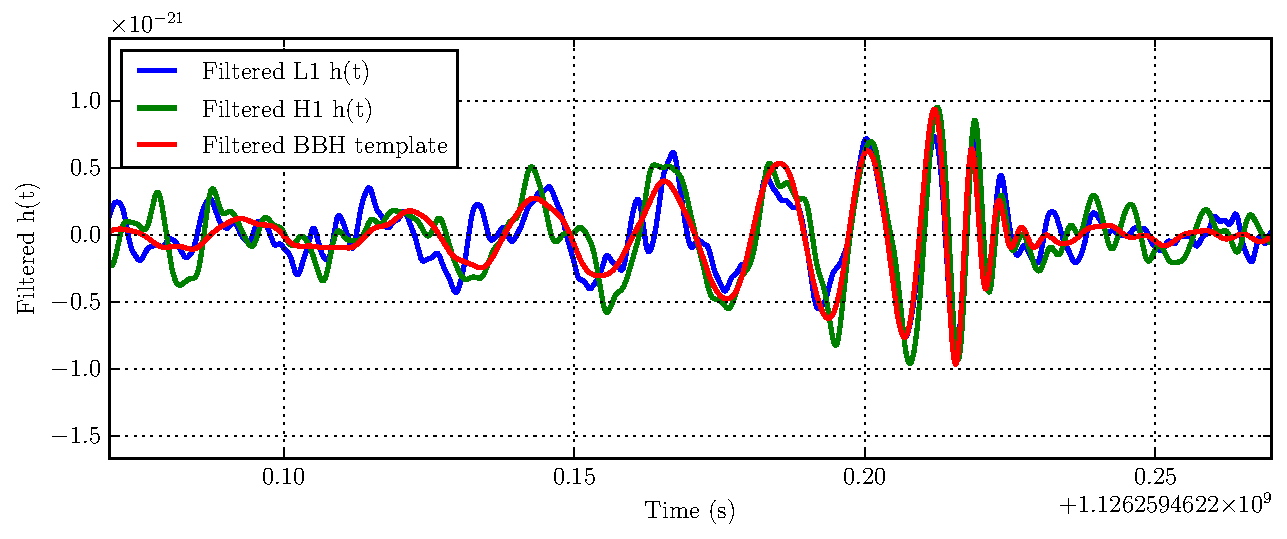
\includegraphics[width=\textwidth]{figures/O1/GW150914-timeseries}
\caption[GW150914 timeseries]{Time-domain representation of L1 %
        gravitational wave strain at the time of GW150914. The blue %
        curve is strain, zero-phase bandpass filtered to isolate the %
        frequencies that contain signal. The red curve is a CBC waveform %
        generated using the best estimated parameters. The CBC waveform %
        has been filtered in the same way as the strain curve.}
\end{figure}\label{fig:GW150914}

We also found GW151226!

LVT151012 was interesting.

\section{PyCBC results}

How significant was GW150914? Figure \ref{fig:pycbc-hist-gw150914} can 
tell us!

\begin{figure}[ht!]%
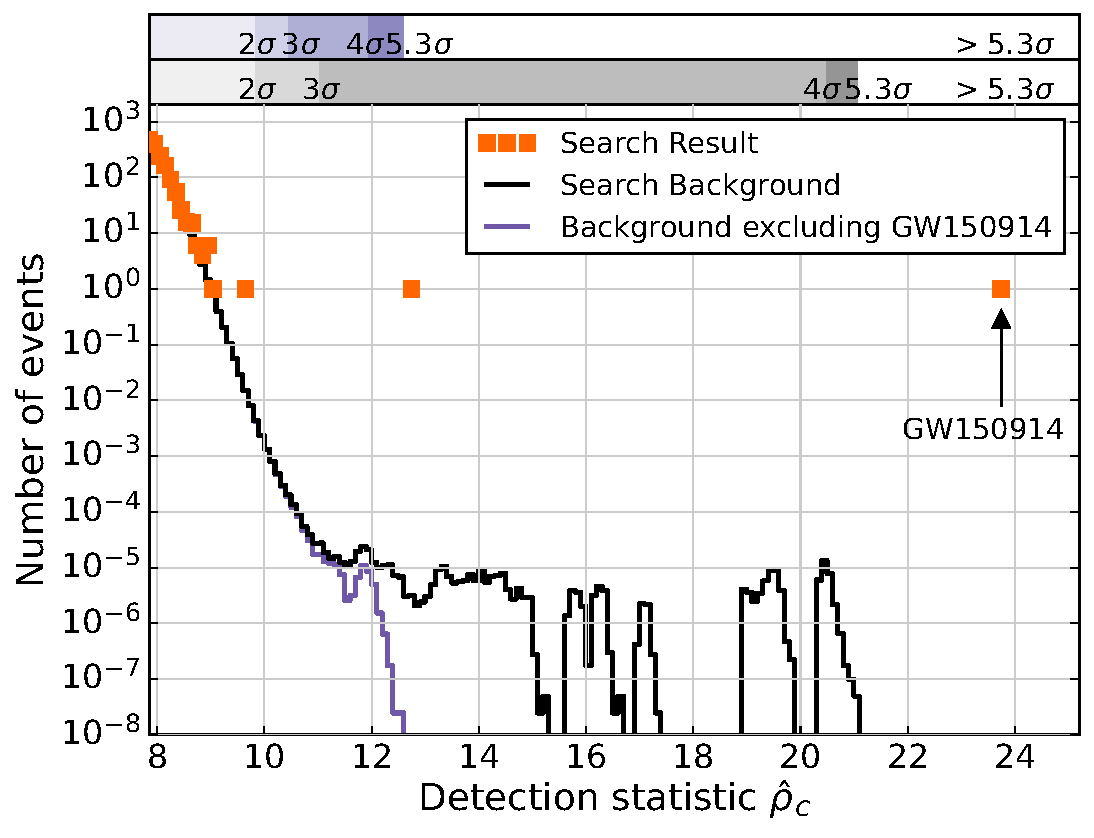
\includegraphics[width=0.8\textwidth]{figures/O1/pycbc_hist_GW150914}
\caption[PyCBC result histograms for GW150914]{Histograms of PyCBC results for GW150914}
\end{figure}\label{fig:pycbc-hist-gw150914}

How significant was GW151226? We have to remove GW150914 to find out. 
Then Figure \ref{fig:pycbc-hist-gw151226} can tell us!

\begin{figure}[ht!]%
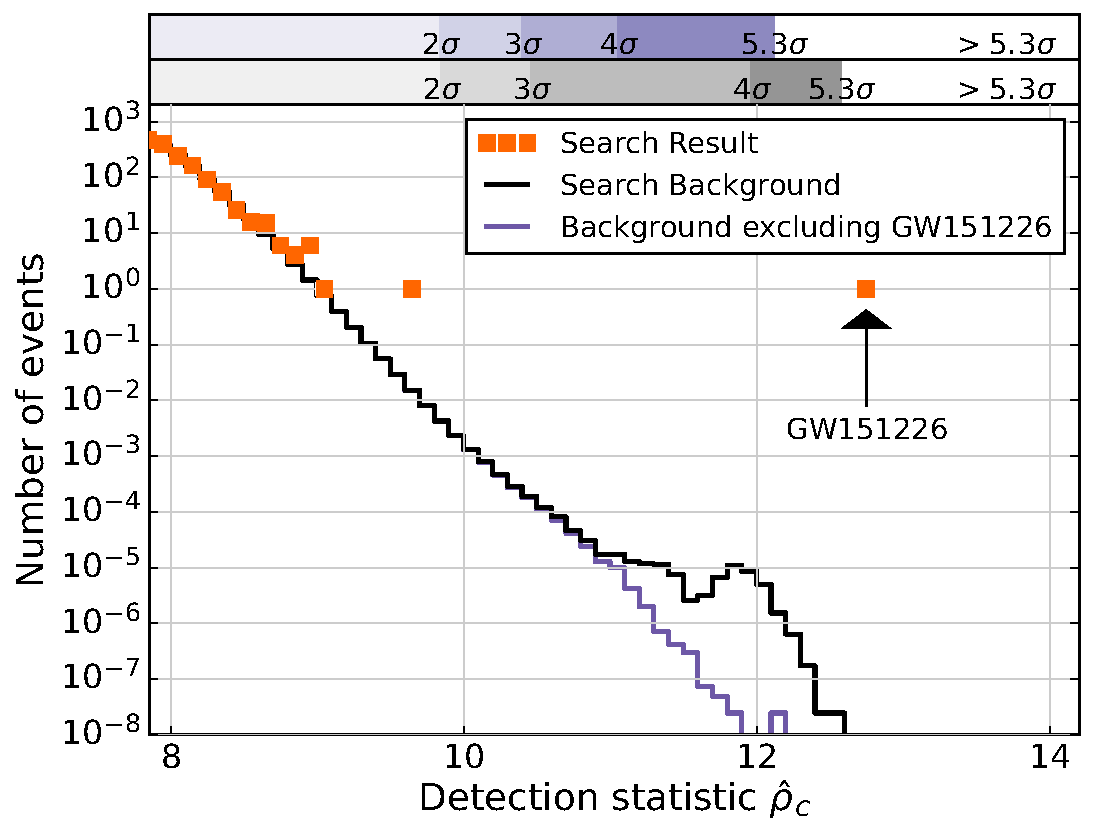
\includegraphics[width=0.8\textwidth]{figures/O1/pycbc_hist_GW151226}
\caption[PyCBC result histograms for GW151226]{Histograms of PyCBC results for GW151226}
\end{figure}\label{fig:pycbc-hist-gw151226}

\begin{table}[ht!]%
  \begin{center}
    \footnotesize
    \begin{tabular}{ccccccc}
    \hline
    Event & Time(UTC) & FAR & $m_1$ ($M_{\odot}$) & $m_2$ ($M_{\odot}$) & $S_{eff}$ & $D_L$ (Mpc) \\
    \hline
    GW150914 & \begin{tabular}{@{}c@{}}14 September \\ 2015 \\ 09:50:45 \end{tabular} & 
    $< 5.8\times10^{-7}$ & $36_{-4}^{+5}$ & $29_{-4}^{+4}$ & $-0.06_{-0.18}^{+0.17}$ & 
    $410_{-180}^{+160}$ \\
    GW151226 & \begin{tabular}{@{}c@{}}26 December \\  2015 \\ 03:38:53 \end{tabular} & 
    $< 5.8\times10^{-7}$ & $14_{-3}^{+9}$ & $8_{-3}^{+2}$ & $0.20_{-0.10}^{+0.21}$ & 
    $490_{-210}^{+180}$ \\
    LVT151226 & \begin{tabular}{@{}c@{}}12 October \\ 2015 \\ 09:54:43 \end{tabular} & 
    0.44 & $23_{-5}^{+18}$ & $13_{-5}^{+4}$ & $0.0_{-0.2}^{+0.3}$ & 
    $1100_{-500}^{+500}$ \\
    \hline
    \end{tabular}
  \end{center}
  \caption[Table of foreground events]{Table of foreground events}
  \label{table:foreground}
\end{table}

